\\[12pt]
\noindent 10. Simule a execução do $\proc{BucketSort}$ com o vetor.

\[ A[1..10] = \langle 0.79, 0.13, 0.16, 0.64, 0.39, 0.20, 0.89, 0.53, 0.71, 0.42 \rangle \]
\\[6pt]
\textbf{Resposta:}
\begin{figure}[h]
  \centering
  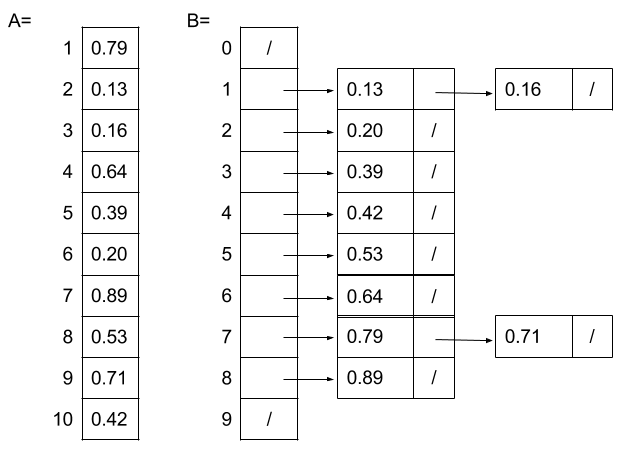
\includegraphics[width=0.7\textwidth]{q5-10}
\end{figure}

\noindent Então cada lista de $B$ é ordenada e concatenada em ordem para gerar o vetor ordenado.